% DOCUMENT
\documentclass[oneside,14pt,a4paper]{extreport}

% LANGUAGE
\usepackage[T2A]{fontenc}
\usepackage[utf8]{inputenc}
\usepackage[english, ukrainian]{babel}

% \usepackage{minted}
\usepackage{pgfplots}

% VARIABLES
\newcommand \labno    {1}
\newcommand \course   {Організація наукових досліджень}
\newcommand \group    {11}
\newcommand \lecturer {Ізонін І. В.}
\newcommand \theme    {Створення облікового запису та наповнення профіля користувача, а також формування рейтингу у Web of Knowledge, Scopus, Google Scholar та ORCID}
\newcommand \purpose  {Створити профілі користувача у Web of Knowlrdge, Scopus, Google Scholar та ORCID. Зрозуміти принципи формування рейтингу у Scopus та Google Scholar.}

% PACKAGES
\usepackage{amssymb}
\usepackage{amsmath}
\usepackage{multirow}
\usepackage{url}

% GEOMETRY
\usepackage{geometry}
\geometry{left   = 2.5cm}
\geometry{right  = 1cm}
\geometry{top    = 2cm}
\geometry{bottom = 2cm}
\renewcommand {\baselinestretch} {1.5}
\setlength\parindent{1cm}

% IMAGES
\usepackage{graphicx}
\usepackage{indentfirst}
\graphicspath{ {./imgs/} }
\usepackage{float}

% FOOTER
\usepackage{fancyhdr}
\fancyhf{}
\renewcommand{\headrulewidth}{0pt}
\cfoot{\hfill \thepage}
\pagestyle{fancy}

% CHAPTERS

\newcommand\Section[1]{
 \refstepcounter{section}
 \section*{
  \arabic{section}. #1}
}

\newcommand\Subsection[1]{
 \refstepcounter{subsection}
 \section*{
  \arabic{section}.\arabic{subsection}. #1}
}

\sloppy
\begin{document}
\begin{titlepage}

\centering
 \textbf{
  МІНІСТЕРСТВО ОСВІТИ І НАУКИ УКРАЇНИ \
  НАЦІОНАЛЬНИЙ УНІВЕРСИТЕТ \flqq{}ЛЬВІВСЬКА ПОЛІТЕХНІКА\frqq{} \
  ІНСТИТУТ КОМП’ЮТЕРНИХ НАУК ТА ІНФОРМАЦІЙНИХ ТЕХНОЛОГІЙ
 }

\vspace{0.5cm}
 \textbf{
  Кафедра систем штучного інтелекту
}

\vspace*{\fill}

  {
    \centering
    
\includegraphics[width=7cm]{imgs/logo.eps}
  }

\vspace{1cm}

  {\textbf{ЗВІТ} \par{}
  {про виконання практичної роботи №\labno}
   \par}
  {з курсу \flqq{}\course\frqq{} \par}

\vspace{1cm} \theme

\raggedleft\vfill

 {\textbf{Виконав:} \par}
 {ст. гр. КНСШ-\group \par}
 {Тимошенко Павло Олександрович \par}

% \vspace{1cm}

 {\textbf{Перевірив:} \par}
 {доцент каф. СШІ, к.т.н.,}
 {\lecturer \par}

\vspace{1cm}

\centering {Львів -- \the\year \par}

\end{titlepage}

\Section{Постановка завдання}

Далі описано пункти, які потрібно виконати у межах цієї практичної роботи.

\begin{enumerate}
    \item Зареєструвати нового користувача у базі Google Scholar. Заповнити усі основні атрибути профілю користувача: додати фото, ПІБ на укр. та англ. мові, університет, ключові слова. Активувати новостворений профіль шляхом підтвердження поштової адреси.
    \item Зареєструвати нового користувача у пошуковій платформі Web of Knowledge. В разі виникнення проблем, це необхідно буде зробити при першій можливості. В цьому випадку, у висновках вказати причини такої ситуації та способи виходу із неї.
    \item Зареєструвати нового користувача у наукометричній базі Scopus. В разі наявності публікацій, які індексуються цією наукометричною базою, вказати їх у звіті. Для пошуку свого, автоматично створеного профілю використати форму пошуку за ПІБ.  
    \item Створити обліковий запис ORCID. Зробити його видимим та активувати. Заповнити необхідні атрибути: місце праці (в разі відсутності місця праці - Університет), місце навчання. Долучити до профілю у поле Websites \& Social Links посилання на Ваш профіль у Google Scholar та на принаймні один профіль у соціальних мережах (наприклад Linkedin чи Facebook). Завантажити та подати у звіті QR-код вашого облікового запису. В разі наявності профілю користувача у Scopus (тобто ПІБ, організація та публікація/публікації) автоматично долучити їх до профіля у ORCID, зв’язавши ці два профілі. Для цього, у Scopus клікнути на Зв’язати з ORCID і виконати усі необхідні подальші кроки.
    \item Описати у звіті усі виконані кроки
\end{enumerate}

\Section{Хід роботи}

Для реєстрації в Google Scholar я створив нового Google-користувача з \flqq{}офіційним\frqq{} адресом електронної пошти. При заповненні профілю в Google Scholar система запропонувала мені налаштувати видимість профілю та параметри оновлення статей. Знімок такого екрану показано на Рис.~\ref{pic:scholar-profile-settings}. Окрім цього я заповнив поля з основною інформацією про профіль. Відповідне вікно показано на Рис.~\ref{pic:scholar-profile-filling}. При створенні профілю обов'язковою опцією було додавання статті до профілю, але оскільки у мене ще немає публікацій, я додав будь-яку, а потім видалив у налаштуваннях профілю. Профіль із невидаленими статтями показано на Рис.~\ref{pic:scholar-profile}, а з видаленими -- на Рис.~\ref{pic:scholar-profile-deleted}. Процедуру пошуку статей продемонстровано на Рис.~\ref{pic:scholar-search}

\begin{figure}[H]
    \centering
    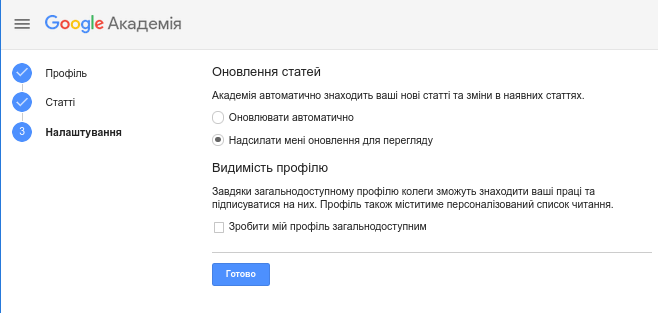
\includegraphics[width=15cm]{imgs/scholar_profile_settings.png}
    \caption{Параметри оновлення статей та налаштування видимості профілю в Google Scholar}
    \label{pic:scholar-profile-settings}
\end{figure}

\begin{figure}[H]
    \centering
    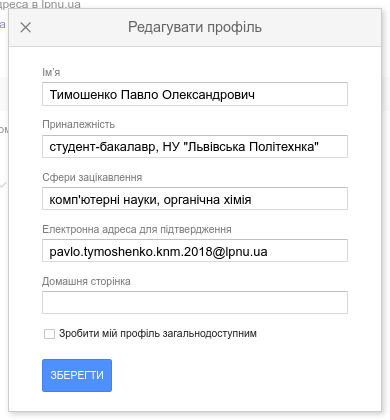
\includegraphics[width=10cm]{imgs/scholar_profile_filling.png}
    \caption{Редагування основної інформації в Google Scholar}
    \label{pic:scholar-profile-filling}
\end{figure}

\begin{figure}[H]
    \centering
    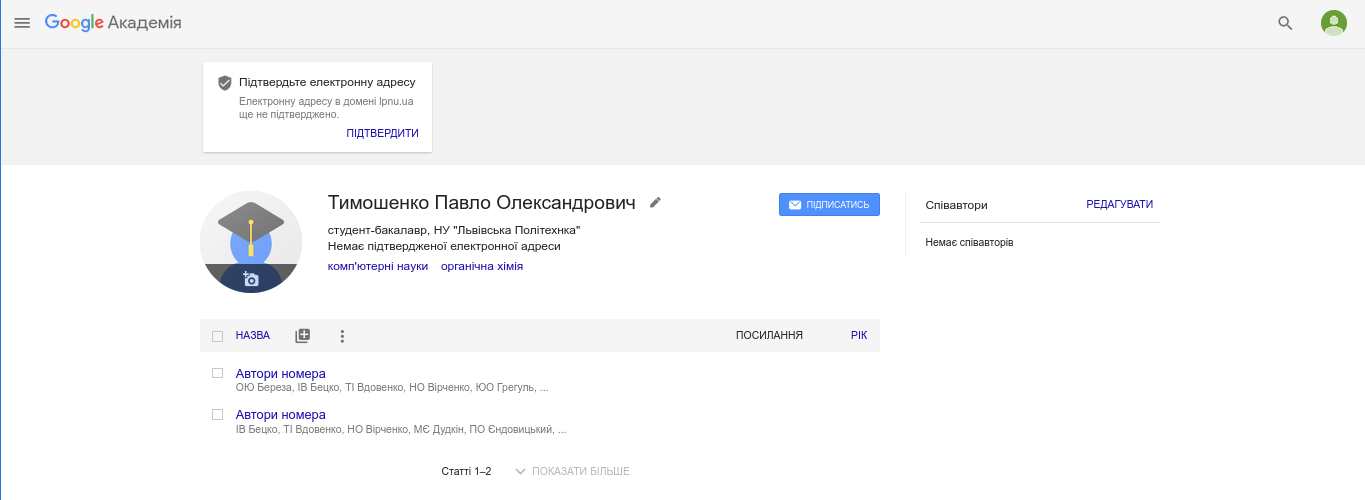
\includegraphics[width=15cm]{imgs/scholar_profile.png}
    \caption{Профіль з невидаленими статтями в Google Scholar}
    \label{pic:scholar-profile}
\end{figure}

\begin{figure}[H]
    \centering
    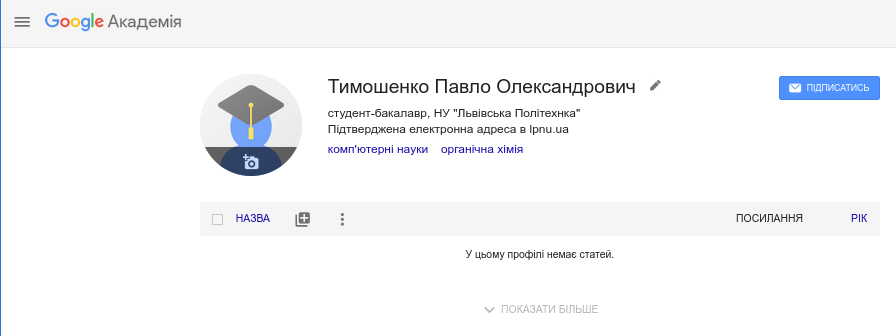
\includegraphics[width=15cm]{imgs/scholar_deleted.png}
    \caption{Профіль з видаленими статтями в Google Scholar}
    \label{pic:scholar-profile-deleted}
\end{figure}

\begin{figure}[H]
    \centering
    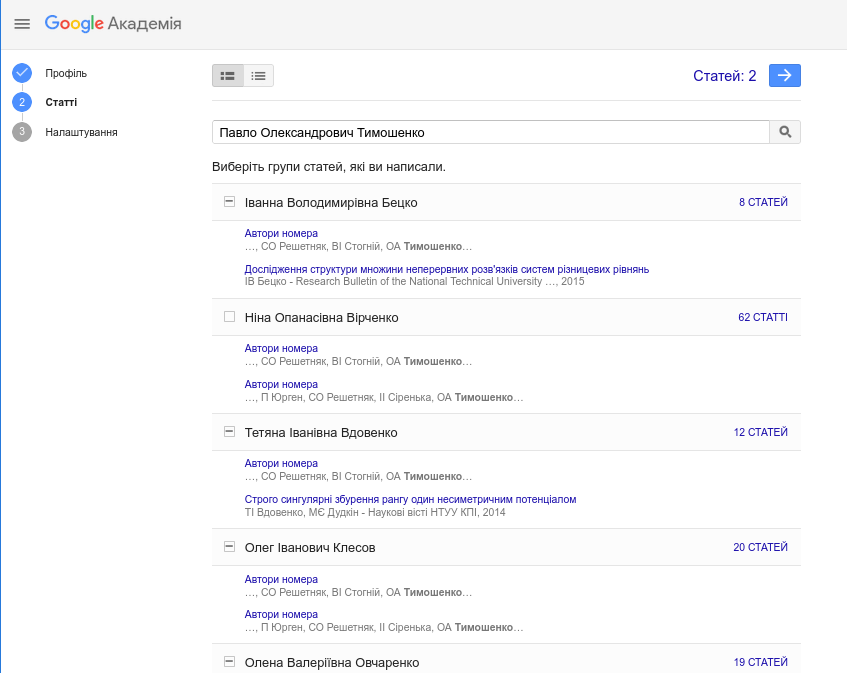
\includegraphics[width=15cm]{imgs/scholar_search.png}
    \caption{Пошук публікацій в Google Scholar}
    \label{pic:scholar-search}
\end{figure}

Мені не вийшло зареєструватись у мережі Web of Science, оскільки я не мав фізичного доступу до мережі Львівської Політехніки, однак я зроблю це за першої можливості.

Окрім цього я зареєструвався у мережі Scopus. Знімок кутоку екрану для неавторизованих користувачів подано на Рис.~\ref{pic:scopus-corner}. Перший крок реєстрації полягає у заповненні спеціальної форми, що зображена на Рис.~\ref{pic:scopus-form}. Після реєстрації облікового запису я отримав можливість переглянути наповнення профілю. Вигляд цього екрану зображено на Рис.~\ref{pic:scopus-account}.

\begin{figure}[H]
    \centering
    
\includegraphics[width=5cm]{imgs/scopus_auth_corner.png}
    \caption{Куточок з кнопкою реєстрації у Scopus}
    \label{pic:scopus-corner}
\end{figure}

\begin{figure}[H]
    \centering
    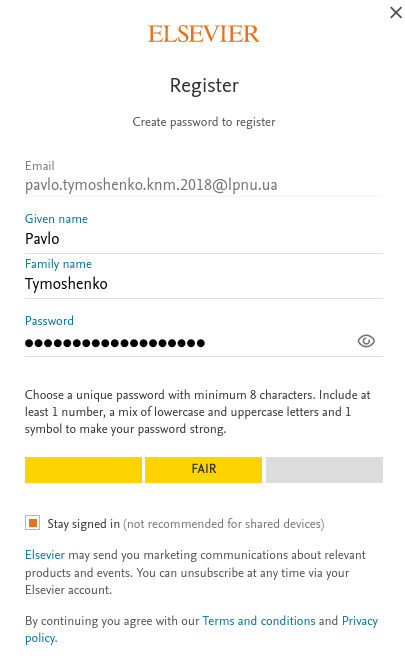
\includegraphics[width=9cm]{imgs/scopus_register_form.png}
    \caption{Форма реєстрації у Scopus}
    \label{pic:scopus-form}
\end{figure}

\begin{figure}[H]
    \centering
    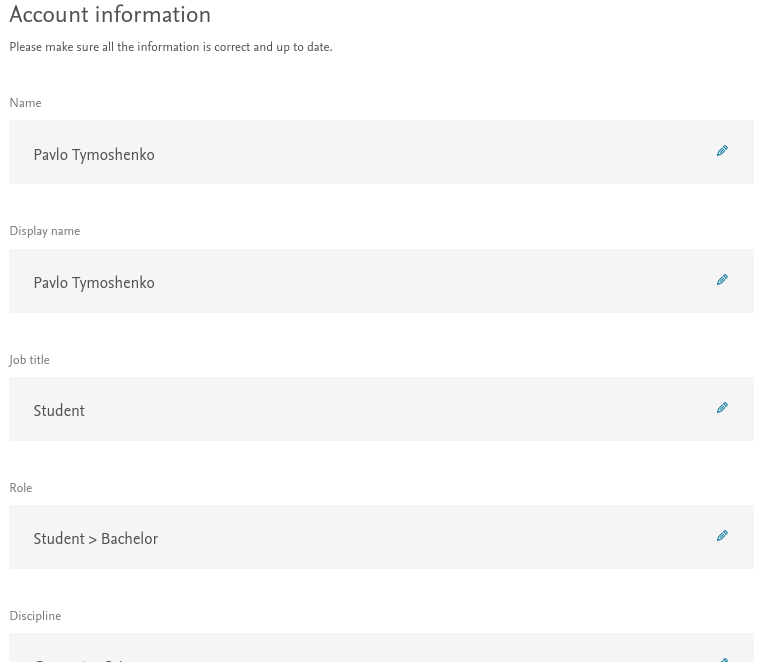
\includegraphics[width=15cm]{imgs/scopus_account.png}
    \caption{Перегляд інформації про користувача Scopus}
    \label{pic:scopus-account}
\end{figure}

Вигляд заповненої форми реєстрації в ORCID показано на Рис.~\ref{pic:orcid-signup-filled}. Також ORCID дозволяє налаштувати видимість профілю. Це зображено на Рис.~\ref{pic:orcid-visibility}. Вигляд заповненого профілю та інформацією про місце навання зображено на Рис.~\ref{pic:orcid-brief} та Рис.~\ref{pic:orcid-biography}.

\begin{figure}[H]
    \centering
    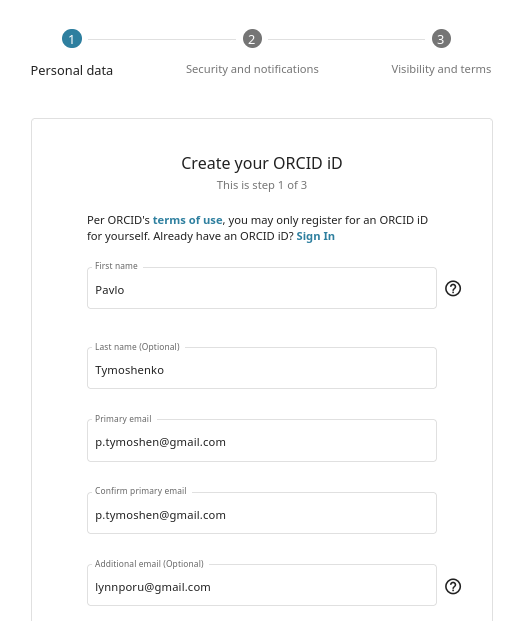
\includegraphics[width=10cm]{imgs/orcid_signup_filled.png}
    \caption{Заповнена форма реєстрації в ORCID}
    \label{pic:orcid-signup-filled}
\end{figure}

\begin{figure}[H]
    \centering
    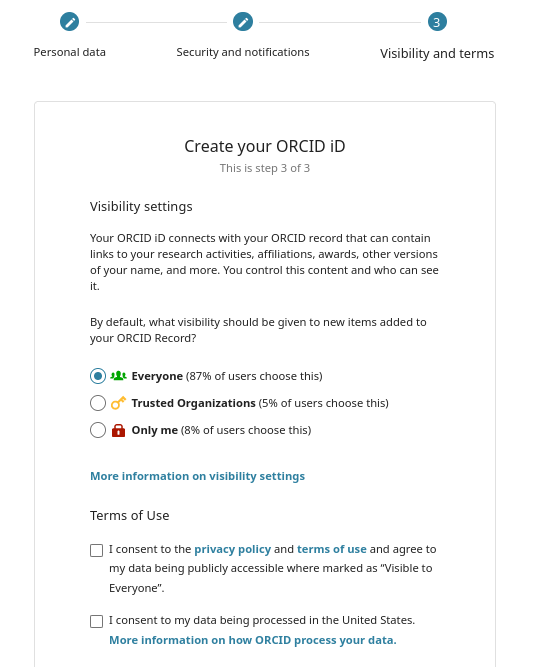
\includegraphics[width=15cm]{imgs/orcid_visibility.png}
    \caption{Налаштування видимості в ORCID}
    \label{pic:orcid-visibility}
\end{figure}

\begin{figure}[H]
    \centering
    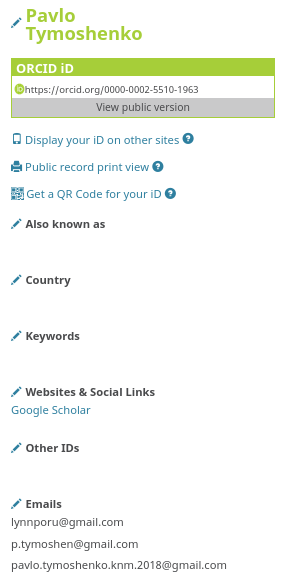
\includegraphics[width=7cm]{imgs/orcid_brief.png}
    \caption{Короткий перегляд профілю в ORCID}
    \label{pic:orcid-brief}
\end{figure}

\begin{figure}[H]
    \centering
    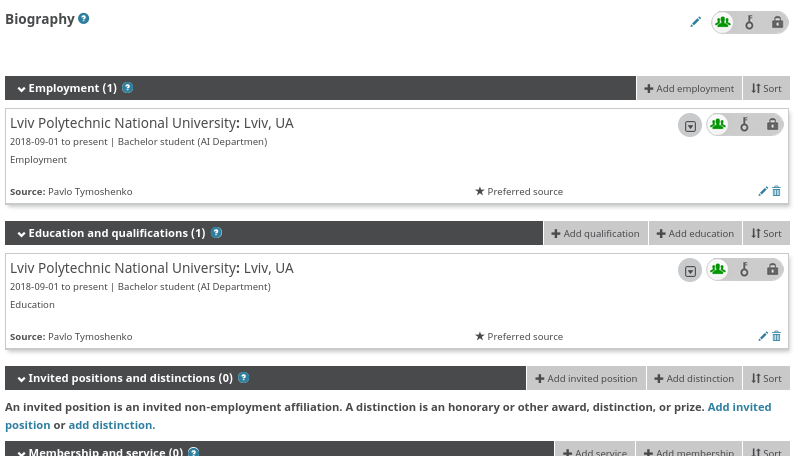
\includegraphics[width=15cm]{imgs/orcid_biography.png}
    \caption{Перегляд біографії в ORCID}
    \label{pic:orcid-biography}
\end{figure}

МОї ідентифікатори у створених наукометричних базах подано у Табл.~\ref{tab:ids}

\begin{table}
    \centering
    \begin{tabular}{|c|c|c|}
        \hline
        №  & Наукометрична база/сервіс   & Ідентифікатор автора      \\ \hline
        1  & Google Scholar              & aYs2\_NUAAAAJ             \\ \hline
        2  & ORCID                       & 0000-0002-5510-1963       \\ \hline
    \end{tabular}
    \caption{Мої ідентифікатори у створених наукометричних базах}
    \label{tab:ids}
\end{table}

\Section{Результати та висновки}

В результаті цієї практичної роботи я створив профілі в Google Scholar, Scopus та ORCID. Також я пов'язав профілі у ORCID та Google Scholar.

\Section{Список використаної літератури}

\begin{enumerate}

\item Пошукова та наукометрична система Гугл Академія (Google Scholar) [Електронний ресурс] – Режим доступу: \url{http://dnsgb.com.ua/files/%D0%A1%D0%98%D0%A1%D0%A2%D0%95%D0%9C%D0%90%20GOOGLE%20%D0%90%D0%9A%D0%90%D0%94%D0%95%D0%9C%D0%86%D0%AF.pdf}  (відвідано 10.10.2020)
\item Веб-адреса бази даних Google Scholar. [Електронний ресурс] – Режим доступу:  \url{https://scholar.google.com/} (відвідано 10.10.2020)
\item База даних Web of Science. Версія 5.22. Інструкція користувачу. [Електронний ресурс] – Режим доступу: \url{http://www.nbuv.gov.ua/sites/default/files/basicpage\_files/201705\_basicpage\_files\_mat/instruction.pdf (відвідано 10.10.2020)/}

\end{enumerate}


\end{document}
